% !Mode:: "TeX:UTF-8"
\chapter{绪论}

如今,多孔圆柱绕流问题成为了人们研究的重要领域,尤其是近年来生物、医学及化学领域的多孔流动问题越来越多,等待着人们更进一步的研究。

\section{圆柱绕流}

在自然界和工程实践中,流体绕过钝体的流动是一种常见的现象。船只在水面行驶,飞行器在空中航行,河水流过桥梁,海水绕过岛屿,风吹过高大的建筑物,这些都是钝体绕流的实例,它出现在我们世界的方方面面,与我们的生活息息相关。人们很早就对这种现象进行了思索和研究,随着流体力学基本理论的建立,人们对此类现象的认识也逐渐深刻起来。

圆柱绕流是流体力学中的一个经典问题,按照雷诺数的划分,整个流动状态可以被划分为许多阶段\cite{Zdravkovich1997b}。在远离圆柱的区域,流动可以按照势流理论处理。在靠近圆柱的区域,按流动特性可以将区域划分为四部分,参见图~\ref{fig: flow area}\cite{demartino2017aerodynamics}。这四个区域可分别称为缓流区、边界层区、边界区和尾迹区。当流体横掠平板时,从平板的前缘开始形成边界层,起初流态为层流状态,随着流体向下游的移动,层流逐渐转变为湍流状态。随着雷诺数的增加,层流转变为湍流的转变区也向上游移动。同样地,当流体流过圆柱时,在下游会出现流态的转变,随着雷诺数的增加,转变点也逐渐向上游移动,并且依次经过划分出来的几个区域,相应的流态称为尾迹区转捩(TrW)、剪切层转捩(TrSL)、边界层转捩(TrBL)。

\begin{figure}[]
	\centering
	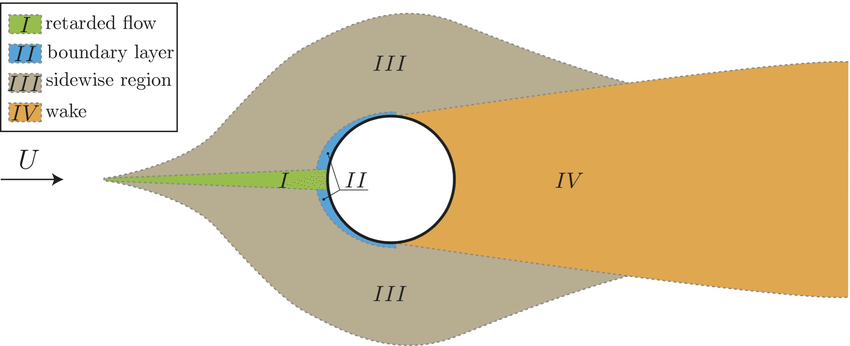
\includegraphics[scale=.4]{figs/Regions-of-disturbed-flow-around-a-perfect-circular-cylinder}
	\caption{流动区域的划分\cite{demartino2017aerodynamics}}
	\label{fig: flow area}
\end{figure}

层流状态(L)。当0 < $Re$ < 4--5时,流体沿着圆柱的轮廓流动,圆柱左右的流线呈现出对称的特性,此时还没有出现流动分离。当4--5 < $Re$ < 30--48时,流体从圆柱表面分离,圆柱的背面开始出现封闭的附着涡,附着涡没有从圆柱表面脱落,此时尚处于稳定状态。当30--48 < $Re$ < 180--200时,圆柱背面的涡从圆柱表面脱落,并由近而远地向远处缓缓飘去。其中在$Re$ > 30--48时,尾迹区逐渐由稳态向非稳态过渡,尾迹末端的流线开始出现类似正弦曲线的摆动。随后,大约在$Re$ > 45--65时,剪切层卷起了一排排的波峰和波谷,接着出现了一列列的涡,即为涡街。

尾迹区转捩(TrW)。这一范围称为亚临界状态。当180--200 < $Re$ < 220--250时,首先在远离圆柱的尾迹区出现层流向湍流的转变(远尾迹转捩,TrW1),随着雷诺数的增大,转变点向上游移动。当220--250 < $Re$ < 350--400时,转变发生在接近圆柱的地方,称为近尾迹转捩(TrW2),最终,当涡一开始产生就已经处于湍流状态。TrW1和TrW2的一个重要现象是非稳态涡产生和脱落的层流模式逐渐被湍流模式所取代\cite{Zdravkovich1997b}。

自由剪切层转捩(TrSL)。雷诺数处于这一范围的流动被称为亚临界状态。当350--400 < $Re$ < 1k--2k时,过渡波首先出现在近壁面剪切层,这一区域称为下亚临界区(TrSL1)。1k--2k < Re < 20k--40k时,过度涡出现在剪切层,在转变为湍流之前,过渡波沿着剪切层卷为分散的涡,之后则继续变成交替的涡,这一阶段为中亚临界区(TrSL2)。雷诺数范围为20k--40k < Re < 100k--200k时是下亚临界区(TrSL3),此时近壁面处已全部转变为湍流状态,近壁面的自由剪切层突然转变为湍流,涡出现在圆柱的背面。

边界层转捩(TrBL)。这一状态也称为临界状态。100k--200k < $Re$ < 300k--340k为前临界区(TrSL0),沿着分离线的剪切层开始转捩,阻力系数开始下降。300k--340k < Re < 380k--400k为单泡临界区(TrBL1),圆柱一侧的自由剪切层重附着形成分离泡。380k--400k < Re < 0.5M--1M为双泡临界区(TrBL2),圆柱两侧形成一对对称的分离泡。0.5M--1M < Re < 3.4M--6M为超临界区(TrBL3),此前出现的分离泡破碎,脱落涡丧失了周期性。3.5M--6M < Re < unknown为过临界区(TrBL4),此时边界层已完全转变为湍流,脱落涡周期性重现。这一阶段雷诺数的上界仍不为人所知。

完全湍流状态(T)。当雷诺数继续增大,整个流场变成了湍流状态。

\section{多孔介质内部的流动}

流体通过多孔介质的流动是地下水水文学、石油工程、土壤学及化学工程等领域的常见现象\cite{Bear2013}。地下水中的含水层,石油工程中的储油层(见图~\ref{fig: Aquifers and oil reservoirs}),以及土壤、多孔岩石、陶瓷、过滤纸和沙过滤器都是多孔介质的实例。此外,流化床、生物过滤器、森林中的降雨、生物工程中的微载体和支架以及多孔换热器也都是多孔介质流动的重要研究领域。

\begin{figure}[]
	\centering
	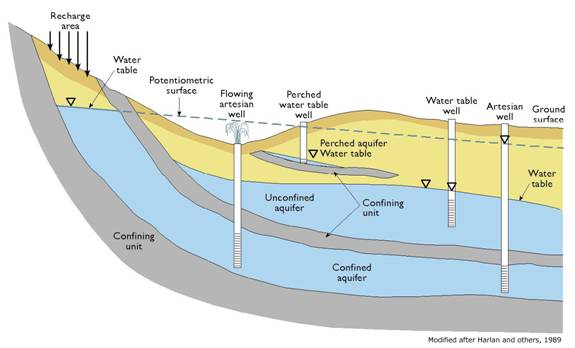
\includegraphics[height=.2\textheight]{figs/Aquifers}
	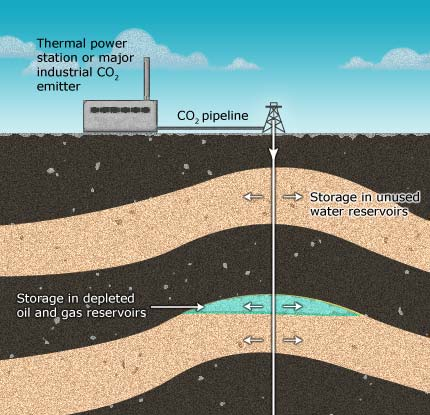
\includegraphics[height=.2\textheight]{figs/Oil-reservoirs}
	\caption{含水层和储油层}
	(图片来源: Colorado Geological Society; Alan Sherwood and Jock Phillips, 'Coal and coal mining - The future of coal', Te Ara - the Encyclopedia of New Zealand)
	\label{fig: Aquifers and oil reservoirs}
\end{figure}

多孔介质可以简单描述为“含有孔洞的固体”,从流体流动的角度来说,它是多相物质占据的空间,且有一相需为固体;固相分布在整个多孔区域;一部分孔隙必须互相连通,使得气液相的流体可以在其中流动\cite{Bear2013}。

流体的连续介质假设将对流体的描述从分子尺度转移到流体质点尺度(微观水平)。类比对流体的描述,我们引入多孔介质的连续介质假设,这样就将描述水平进一步转到表征体积单元(REV)的尺度上(宏观水平)。在这个假设的基础上,我们可以用连续函数来描述多孔介质内的流动,并由此建立起相应的质量方程和动量方程。

\section{绕过及穿过多孔钝体的流动}

\section{研究问题和文章结构}
